\documentclass{article}\usepackage[]{graphicx}\usepackage[]{color}
%% maxwidth is the original width if it is less than linewidth
%% otherwise use linewidth (to make sure the graphics do not exceed the margin)
\makeatletter
\def\maxwidth{ %
  \ifdim\Gin@nat@width>\linewidth
    \linewidth
  \else
    \Gin@nat@width
  \fi
}
\makeatother

\definecolor{fgcolor}{rgb}{0.345, 0.345, 0.345}
\newcommand{\hlnum}[1]{\textcolor[rgb]{0.686,0.059,0.569}{#1}}%
\newcommand{\hlstr}[1]{\textcolor[rgb]{0.192,0.494,0.8}{#1}}%
\newcommand{\hlcom}[1]{\textcolor[rgb]{0.678,0.584,0.686}{\textit{#1}}}%
\newcommand{\hlopt}[1]{\textcolor[rgb]{0,0,0}{#1}}%
\newcommand{\hlstd}[1]{\textcolor[rgb]{0.345,0.345,0.345}{#1}}%
\newcommand{\hlkwa}[1]{\textcolor[rgb]{0.161,0.373,0.58}{\textbf{#1}}}%
\newcommand{\hlkwb}[1]{\textcolor[rgb]{0.69,0.353,0.396}{#1}}%
\newcommand{\hlkwc}[1]{\textcolor[rgb]{0.333,0.667,0.333}{#1}}%
\newcommand{\hlkwd}[1]{\textcolor[rgb]{0.737,0.353,0.396}{\textbf{#1}}}%
\let\hlipl\hlkwb

\usepackage{framed}
\makeatletter
\newenvironment{kframe}{%
 \def\at@end@of@kframe{}%
 \ifinner\ifhmode%
  \def\at@end@of@kframe{\end{minipage}}%
  \begin{minipage}{\columnwidth}%
 \fi\fi%
 \def\FrameCommand##1{\hskip\@totalleftmargin \hskip-\fboxsep
 \colorbox{shadecolor}{##1}\hskip-\fboxsep
     % There is no \\@totalrightmargin, so:
     \hskip-\linewidth \hskip-\@totalleftmargin \hskip\columnwidth}%
 \MakeFramed {\advance\hsize-\width
   \@totalleftmargin\z@ \linewidth\hsize
   \@setminipage}}%
 {\par\unskip\endMakeFramed%
 \at@end@of@kframe}
\makeatother

\definecolor{shadecolor}{rgb}{.97, .97, .97}
\definecolor{messagecolor}{rgb}{0, 0, 0}
\definecolor{warningcolor}{rgb}{1, 0, 1}
\definecolor{errorcolor}{rgb}{1, 0, 0}
\newenvironment{knitrout}{}{} % an empty environment to be redefined in TeX

\usepackage{alltt}

\usepackage{amsmath, amssymb}
\usepackage{graphicx}
\usepackage{hyperref}
\usepackage{listings}
\IfFileExists{upquote.sty}{\usepackage{upquote}}{}
\begin{document}

\title{Pol Sci 630:  Problem Set 12 Solutions: 2SLS, RDD, ggplot2}

\author{Prepared by: Anh Le (\href{mailto:anh.le@duke.edu}{anh.le@duke.edu})}

\date{Due Date: Friday, Nov 23, 2016 (Beginning of Class)}

\maketitle

\section{2SLS}

\textbf{\color{red} Insert your comments on the assignment that you are grading above the solution in bold and red text. For example write: "GRADER COMMENT: everything is correct! - 8/8 Points" Also briefly point out which, if any, problems were not solved correctly and what the mistake was. See below for more examples.}

\subsection{Load dataset CigarettesSW from package AER}

\begin{knitrout}
\definecolor{shadecolor}{rgb}{0.969, 0.969, 0.969}\color{fgcolor}\begin{kframe}
\begin{alltt}
\hlkwd{library}\hlstd{(AER)}
\hlkwd{data}\hlstd{(}\hlstr{"CigarettesSW"}\hlstd{)}
\end{alltt}
\end{kframe}
\end{knitrout}

\subsection{Plot the following using ggplot2}

What can we say about the relationship between tax, price, and packs? Importantly, could sales tax be a valid instrument here? Explain your reasoning.

Note: This is a good way to show the relationship between 3 variables with a 2D plot.

\begin{knitrout}
\definecolor{shadecolor}{rgb}{0.969, 0.969, 0.969}\color{fgcolor}
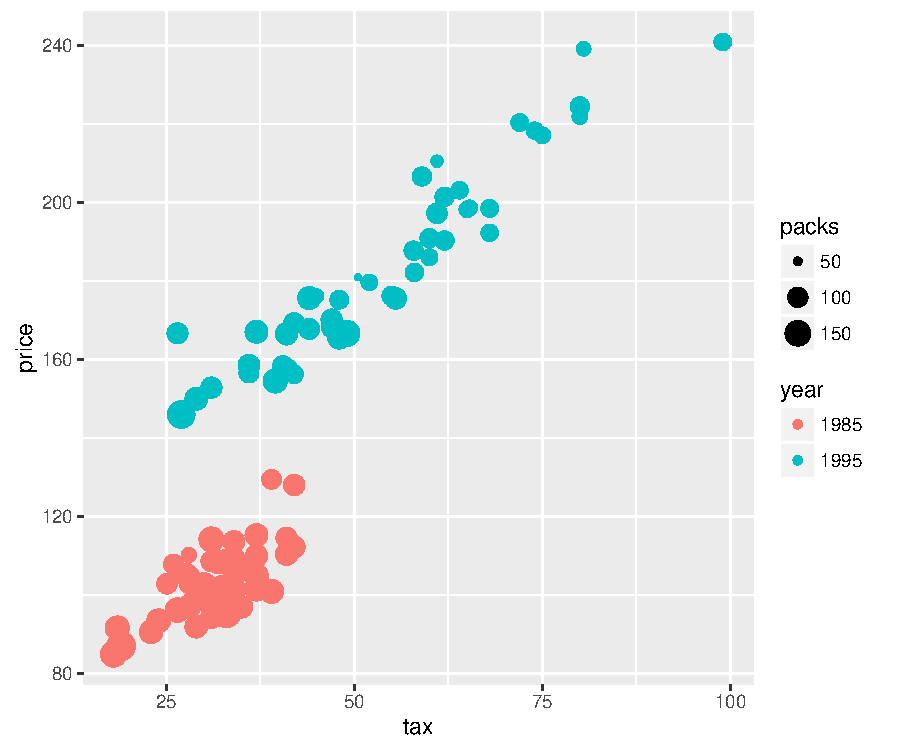
\includegraphics[width=\maxwidth]{figure/unnamed-chunk-2-1} 

\end{knitrout}

\textbf{Solution}

For tax to be a good instrument, it has to 1) correlate with price, 2) not correlate with some other factors that affect packs (i.e. not endogenous).

Criterion (1) seems satisfied as the plot shows a positive correlation between tax and price. Whether (2) is satisfied is unclear. On the one hand, if tax is a cigarette-specific tax, it's likely that there's a reverse causality problem as legislators expect more cigarette consumption and raise tax to counter it. In this case, tax is not a valid instrument. On the other hand, if tax is some general sales tax, it's possible that it's changed based on some other factors unrelated to cigarette. In this case, tax is a valid instrument.

Tax and price are negatively correlated with the number of cigarette packs consumed per capita.

\subsection{Divide variable income by 1000 (for interpretability)}

\begin{knitrout}
\definecolor{shadecolor}{rgb}{0.969, 0.969, 0.969}\color{fgcolor}\begin{kframe}
\begin{alltt}
\hlstd{CigarettesSW}\hlopt{$}\hlstd{income} \hlkwb{<-} \hlstd{CigarettesSW}\hlopt{$}\hlstd{income} \hlopt{/} \hlnum{1000}
\end{alltt}
\end{kframe}
\end{knitrout}


\subsection{Run 2SLS}

Run 2SLS with \verb`ivreg`. Outcome: packs. Exogenous var: income. Endogenous var: price, whose instrument is tax. Interpret the coefficient of \verb`income` and \verb`price`.

Note: Different from the model during lab, this model has an exogenous independent variable that doesn't need to be instrumented for. See `help(ivreg)` $>$ Details, which explains how to deal with this.

\textbf{Solution}

\begin{kframe}
\begin{alltt}
\hlkwd{library}\hlstd{(stargazer)}
\hlstd{m11} \hlkwb{<-} \hlkwd{ivreg}\hlstd{(packs} \hlopt{~} \hlstd{income} \hlopt{+} \hlstd{price} \hlopt{|} \hlstd{income} \hlopt{+} \hlstd{tax,} \hlkwc{data} \hlstd{= CigarettesSW)}
\hlkwd{stargazer}\hlstd{(m11)}
\end{alltt}
\end{kframe}
% Table created by stargazer v.5.2 by Marek Hlavac, Harvard University. E-mail: hlavac at fas.harvard.edu
% Date and time: Fri, Nov 18, 2016 - 07:14:10 PM
\begin{table}[!htbp] \centering 
  \caption{} 
  \label{} 
\begin{tabular}{@{\extracolsep{5pt}}lc} 
\\[-1.8ex]\hline 
\hline \\[-1.8ex] 
 & \multicolumn{1}{c}{\textit{Dependent variable:}} \\ 
\cline{2-2} 
\\[-1.8ex] & packs \\ 
\hline \\[-1.8ex] 
 income & $-$0.00002 \\ 
  & (0.00002) \\ 
  & \\ 
 price & $-$0.398$^{***}$ \\ 
  & (0.055) \\ 
  & \\ 
 Constant & 168.488$^{***}$ \\ 
  & (7.673) \\ 
  & \\ 
\hline \\[-1.8ex] 
Observations & 96 \\ 
R$^{2}$ & 0.436 \\ 
Adjusted R$^{2}$ & 0.424 \\ 
Residual Std. Error & 19.637 (df = 93) \\ 
\hline 
\hline \\[-1.8ex] 
\textit{Note:}  & \multicolumn{1}{r}{$^{*}$p$<$0.1; $^{**}$p$<$0.05; $^{***}$p$<$0.01} \\ 
\end{tabular} 
\end{table} 


1000 dollar increase in income per capita leads to \ensuremath{-2.2311969\times 10^{-5}} change in number of packs per capita, but the effect is not significant.

1 dollar increase in price leads to \ensuremath{-0.3978933} change in number of packs per capita, holding others constant. The coefficient is statistically significant.

\subsection{2SLS diagnostics: use F-test to check for weak instrument}

\textbf{Solution}

\begin{knitrout}
\definecolor{shadecolor}{rgb}{0.969, 0.969, 0.969}\color{fgcolor}\begin{kframe}
\begin{alltt}
\hlkwd{summary}\hlstd{(m11,} \hlkwc{diagnostics} \hlstd{=} \hlnum{TRUE}\hlstd{)}
\end{alltt}
\begin{verbatim}
## 
## Call:
## ivreg(formula = packs ~ income + price | income + tax, data = CigarettesSW)
## 
## Residuals:
##       Min        1Q    Median        3Q       Max 
## -56.16120 -10.40243   0.07866   6.87649  67.85671 
## 
## Coefficients:
##               Estimate Std. Error t value Pr(>|t|)    
## (Intercept)  1.685e+02  7.673e+00  21.957  < 2e-16 ***
## income      -2.231e-05  1.803e-05  -1.238    0.219    
## price       -3.979e-01  5.502e-02  -7.232 1.31e-10 ***
## 
## Diagnostic tests:
##                  df1 df2 statistic p-value    
## Weak instruments   1  93   341.145  <2e-16 ***
## Wu-Hausman         1  92     2.312   0.132    
## Sargan             0  NA        NA      NA    
## ---
## Signif. codes:  0 '***' 0.001 '**' 0.01 '*' 0.05 '.' 0.1 ' ' 1
## 
## Residual standard error: 19.64 on 93 degrees of freedom
## Multiple R-Squared: 0.436,	Adjusted R-squared: 0.4239 
## Wald test: 35.23 on 2 and 93 DF,  p-value: 4.081e-12
\end{verbatim}
\end{kframe}
\end{knitrout}

The weak instrument test (i.e. F-test) rejects the null hypothesis that the instrument is not correlated with the endogenous variable (p-value = \ensuremath{7.1137017\times 10^{-33}}). So our instruments are not weak.

\subsection{2SLS by hand}

Run the 2SLS by hand, i.e. not using \verb`ivreg`, but run 2 stages of \verb`lm`. Do you get the same estimate from \verb`ivreg`?

\textbf{Solution}

\begin{kframe}
\begin{alltt}
\hlstd{m_stage1} \hlkwb{<-} \hlkwd{lm}\hlstd{(price} \hlopt{~} \hlstd{tax} \hlopt{+} \hlstd{income,} \hlkwc{data} \hlstd{= CigarettesSW)}
\hlstd{CigarettesSW}\hlopt{$}\hlstd{price_hat} \hlkwb{<-} \hlkwd{predict}\hlstd{(m_stage1)}

\hlstd{m_stage2} \hlkwb{<-} \hlkwd{lm}\hlstd{(packs} \hlopt{~} \hlstd{income} \hlopt{+} \hlstd{price_hat,} \hlkwc{data} \hlstd{= CigarettesSW)}
\hlkwd{stargazer}\hlstd{(m_stage2)}
\end{alltt}
\end{kframe}
% Table created by stargazer v.5.2 by Marek Hlavac, Harvard University. E-mail: hlavac at fas.harvard.edu
% Date and time: Fri, Nov 18, 2016 - 07:14:11 PM
\begin{table}[!htbp] \centering 
  \caption{} 
  \label{} 
\begin{tabular}{@{\extracolsep{5pt}}lc} 
\\[-1.8ex]\hline 
\hline \\[-1.8ex] 
 & \multicolumn{1}{c}{\textit{Dependent variable:}} \\ 
\cline{2-2} 
\\[-1.8ex] & packs \\ 
\hline \\[-1.8ex] 
 income & $-$0.00002 \\ 
  & (0.00002) \\ 
  & \\ 
 price\_hat & $-$0.398$^{***}$ \\ 
  & (0.055) \\ 
  & \\ 
 Constant & 168.488$^{***}$ \\ 
  & (7.733) \\ 
  & \\ 
\hline \\[-1.8ex] 
Observations & 96 \\ 
R$^{2}$ & 0.427 \\ 
Adjusted R$^{2}$ & 0.415 \\ 
Residual Std. Error & 19.788 (df = 93) \\ 
F Statistic & 34.693$^{***}$ (df = 2; 93) \\ 
\hline 
\hline \\[-1.8ex] 
\textit{Note:}  & \multicolumn{1}{r}{$^{*}$p$<$0.1; $^{**}$p$<$0.05; $^{***}$p$<$0.01} \\ 
\end{tabular} 
\end{table} 


The coefficients are exactly the same (by hand: \ensuremath{-0.3978933}, by ivreg: \ensuremath{-0.3978933})

\subsection{Weak instrument test by hand}

The weak instrument test aims to test whether the instrument is an important predictor of the endogenous variables, even after controlling for other variables.

We do it as follows:

\begin{itemize}
\item Run the standard 1st stage regression of endogenous var ~ instrument + exogenous vars
\item Run a ``modified'' 1st stage regression of endogenous var ~ exogenous vars
\item Use \verb`waldtest(model1, model2)` to compare the two models (to see if the model with the instrument fits better). The null hypothesis is that the instrument has a statistically significant impact
\end{itemize}
The rule of thumb is that the F-statistic should be $>$ 10

Implement the weak instrument test as described above and show that it gets the same F-statistic as given by \verb`ivreg`.

\textbf{Solution}

\begin{knitrout}
\definecolor{shadecolor}{rgb}{0.969, 0.969, 0.969}\color{fgcolor}\begin{kframe}
\begin{alltt}
\hlstd{m_stage1_without_instrument} \hlkwb{<-} \hlkwd{lm}\hlstd{(price} \hlopt{~} \hlstd{income,} \hlkwc{data} \hlstd{= CigarettesSW)}
\hlstd{(t_wald} \hlkwb{<-} \hlkwd{waldtest}\hlstd{(m_stage1, m_stage1_without_instrument))}
\end{alltt}
\begin{verbatim}
## Wald test
## 
## Model 1: price ~ tax + income
## Model 2: price ~ income
##   Res.Df Df      F    Pr(>F)    
## 1     93                        
## 2     94 -1 341.14 < 2.2e-16 ***
## ---
## Signif. codes:  0 '***' 0.001 '**' 0.01 '*' 0.05 '.' 0.1 ' ' 1
\end{verbatim}
\end{kframe}
\end{knitrout}

The F-statistic the same (by hand: 341.1446676, by ivreg: 341.1446676).

\section{Regression Discontinuity Design}

Find the replication data here \url{https://dataverse.harvard.edu/dataset.xhtml?persistentId=doi:10.7910/DVN/9OOLQ7}

\begin{knitrout}
\definecolor{shadecolor}{rgb}{0.969, 0.969, 0.969}\color{fgcolor}\begin{kframe}
\begin{alltt}
\hlkwd{load}\hlstd{(}\hlstr{"replication_data.RData"}\hlstd{)}
\end{alltt}
\end{kframe}
\end{knitrout}

Variables that you'll use: elecpopratio (\% of the population as the electorate), treat (whether got audited or not), electorate.perpop07 (\% registration in 07), electorate.perpop08 (\% registration in 08)

Read (by which I mean Ctrl + F) through the paper to figure out which bandwidth and the cutoff points the authors used. Read help(rdrobust) to see how to specify our own bandwidth and cutoff points.

In this exercise we'll replicate their main results in Table 2 (p. 447)

\subsection{Sharp RDD}

Use rdrobust to estimate the RDD effect of elecpopratio $>$ 0.8 for Change in registration (\%) ($\hat\tau_A$ in Table 2), using 1) the author's bandwidth, and 2) the bandwidth chosen by rdrobust itself.

\textbf{Solution}

\begin{knitrout}
\definecolor{shadecolor}{rgb}{0.969, 0.969, 0.969}\color{fgcolor}\begin{kframe}
\begin{alltt}
\hlkwd{library}\hlstd{(rdrobust)}
\hlcom{# Author's bandwidth}
\hlkwd{rdrobust}\hlstd{(}\hlkwc{y} \hlstd{= data}\hlopt{$}\hlstd{electorate.perpop08} \hlopt{-} \hlstd{data}\hlopt{$}\hlstd{electorate.perpop07,}
        \hlkwc{x} \hlstd{= data}\hlopt{$}\hlstd{elecpopratio,}
        \hlkwc{c} \hlstd{=} \hlnum{0.8}\hlstd{,} \hlkwc{h} \hlstd{=} \hlnum{0.04}\hlstd{,} \hlkwc{all} \hlstd{=} \hlnum{TRUE}\hlstd{)}
\end{alltt}
\begin{verbatim}
## Call:
## rdrobust(y = data$electorate.perpop08 - data$electorate.perpop07, 
##     x = data$elecpopratio, c = 0.8, h = 0.04, all = TRUE)
## 
## Summary:
##                         
## Number of Obs 5476      
## BW Type       Manual    
## Kernel Type   Triangular
## VCE Type      NN        
## 
##                    Left   Right 
## Number of Obs      4013   1463  
## Eff. Number of Obs 850    605   
## Order Loc Poly (p) 1      1     
## Order Bias (q)     2      2     
## BW Loc Poly (h)    0.0400 0.0400
## BW Bias (b)        0.0400 0.0400
## rho (h/b)          1.0000 1.0000
## 
## Estimates:
##                Coef    Std. Err. z        P>|z|  CI Lower CI Upper
## Conventional   -9.5193 0.6997    -13.6043 0.0000 -10.8907 -8.1479 
## Bias-Corrected -9.8630 0.6997    -14.0955 0.0000 -11.2344 -8.4916 
## Robust         -9.8630 0.9506    -10.3751 0.0000 -11.7262 -7.9998
\end{verbatim}
\begin{alltt}
\hlcom{# Auto bandwidth}
\hlkwd{rdrobust}\hlstd{(}\hlkwc{y} \hlstd{= data}\hlopt{$}\hlstd{electorate.perpop08} \hlopt{-} \hlstd{data}\hlopt{$}\hlstd{electorate.perpop07,}
                       \hlkwc{x} \hlstd{= data}\hlopt{$}\hlstd{elecpopratio,} \hlkwc{c} \hlstd{=} \hlnum{0.8}\hlstd{,} \hlkwc{all} \hlstd{=} \hlnum{TRUE}\hlstd{)}
\end{alltt}
\begin{verbatim}
## Call:
## rdrobust(y = data$electorate.perpop08 - data$electorate.perpop07, 
##     x = data$elecpopratio, c = 0.8, all = TRUE)
## 
## Summary:
##                         
## Number of Obs 5476      
## BW Type       mserd     
## Kernel Type   Triangular
## VCE Type      NN        
## 
##                    Left   Right 
## Number of Obs      4013   1463  
## Eff. Number of Obs 1372   836   
## Order Loc Poly (p) 1      1     
## Order Bias (q)     2      2     
## BW Loc Poly (h)    0.0622 0.0622
## BW Bias (b)        0.1339 0.1339
## rho (h/b)          0.4642 0.4642
## 
## Estimates:
##                Coef    Std. Err. z        P>|z|  CI Lower CI Upper
## Conventional   -9.1917 0.5921    -15.5236 0.0000 -10.3522 -8.0312 
## Bias-Corrected -9.4370 0.5921    -15.9380 0.0000 -10.5976 -8.2765 
## Robust         -9.4370 0.6502    -14.5139 0.0000 -10.7114 -8.1627
\end{verbatim}
\end{kframe}
\end{knitrout}

The effect sizes of the two models are about the same as the paper's.

\subsection{Fuzzy RDD}

The design of this paper is a Fuzzy RDD because when elecpopratio $>$ 0.8, a district may be audited but not necessarily.

rdrobust has an argument \verb`fuzzy` to specify which observation is actually treated. Use it to get a Fuzzy RDD estimate for Change in registration (\%) ($\hat\tau_R$ in Table 2)

\textbf{Solution}

\begin{knitrout}
\definecolor{shadecolor}{rgb}{0.969, 0.969, 0.969}\color{fgcolor}\begin{kframe}
\begin{alltt}
\hlcom{# Author's bandwidth}
\hlkwd{rdrobust}\hlstd{(}\hlkwc{y} \hlstd{= data}\hlopt{$}\hlstd{electorate.perpop08} \hlopt{-} \hlstd{data}\hlopt{$}\hlstd{electorate.perpop07,}
        \hlkwc{x} \hlstd{= data}\hlopt{$}\hlstd{elecpopratio,}
        \hlkwc{fuzzy} \hlstd{= data}\hlopt{$}\hlstd{treat,}
        \hlkwc{c} \hlstd{=} \hlnum{0.8}\hlstd{,} \hlkwc{h} \hlstd{=} \hlnum{0.04}\hlstd{,} \hlkwc{all} \hlstd{=} \hlnum{TRUE}\hlstd{)}
\end{alltt}
\begin{verbatim}
## Call:
## rdrobust(y = data$electorate.perpop08 - data$electorate.perpop07, 
##     x = data$elecpopratio, fuzzy = data$treat, c = 0.8, h = 0.04, 
##     all = TRUE)
## 
## Summary:
##                         
## Number of Obs 5476      
## BW Type       Manual    
## Kernel Type   Triangular
## VCE Type      NN        
## 
##                    Left   Right 
## Number of Obs      4013   1463  
## Eff. Number of Obs 850    605   
## Order Loc Poly (p) 1      1     
## Order Bias (q)     2      2     
## BW Loc Poly (h)    0.0400 0.0400
## BW Bias (b)        0.0400 0.0400
## rho (h/b)          1.0000 1.0000
## 
## Estimates:
##                Coef     Std. Err. z        P>|z|  CI Lower CI Upper
## Conventional   -12.8448 0.7361    -17.4510 0.0000 -14.2875 -11.4022
## Bias-Corrected -13.1578 0.7361    -17.8761 0.0000 -14.6004 -11.7151
## Robust         -13.1578 0.9761    -13.4797 0.0000 -15.0709 -11.2446
\end{verbatim}
\begin{alltt}
\hlcom{# Auto bandwidth}
\hlkwd{rdrobust}\hlstd{(}\hlkwc{y} \hlstd{= data}\hlopt{$}\hlstd{electorate.perpop08} \hlopt{-} \hlstd{data}\hlopt{$}\hlstd{electorate.perpop07,}
         \hlkwc{fuzzy} \hlstd{= data}\hlopt{$}\hlstd{treat,}
         \hlkwc{x} \hlstd{= data}\hlopt{$}\hlstd{elecpopratio,} \hlkwc{c} \hlstd{=} \hlnum{0.8}\hlstd{,} \hlkwc{all} \hlstd{=} \hlnum{TRUE}\hlstd{)}
\end{alltt}
\begin{verbatim}
## Call:
## rdrobust(y = data$electorate.perpop08 - data$electorate.perpop07, 
##     x = data$elecpopratio, fuzzy = data$treat, c = 0.8, all = TRUE)
## 
## Summary:
##                         
## Number of Obs 5476      
## BW Type       mserd     
## Kernel Type   Triangular
## VCE Type      NN        
## 
##                    Left   Right 
## Number of Obs      4013   1463  
## Eff. Number of Obs 938    657   
## Order Loc Poly (p) 1      1     
## Order Bias (q)     2      2     
## BW Loc Poly (h)    0.0445 0.0445
## BW Bias (b)        0.1060 0.1060
## rho (h/b)          0.4195 0.4195
## 
## Estimates:
##                Coef     Std. Err. z        P>|z|  CI Lower CI Upper
## Conventional   -12.7913 0.7134    -17.9310 0.0000 -14.1895 -11.3932
## Bias-Corrected -13.0176 0.7134    -18.2482 0.0000 -14.4158 -11.6194
## Robust         -13.0176 0.7646    -17.0253 0.0000 -14.5162 -11.5190
\end{verbatim}
\end{kframe}
\end{knitrout}

The paper's estimate is 11.93, pretty close.

\subsection{Density test (graphical)}

Plot the histogram of the number of observations on both sides of the cut-off to see if there's any difference

\textbf{Solution}

\begin{knitrout}
\definecolor{shadecolor}{rgb}{0.969, 0.969, 0.969}\color{fgcolor}\begin{kframe}
\begin{alltt}
\hlkwd{ggplot}\hlstd{(}\hlkwc{data} \hlstd{= data)} \hlopt{+}
  \hlkwd{geom_histogram}\hlstd{(}\hlkwd{aes}\hlstd{(}\hlkwc{x} \hlstd{= elecpopratio,} \hlkwc{fill} \hlstd{=} \hlkwd{factor}\hlstd{(elecpopratio} \hlopt{>} \hlnum{0.8}\hlstd{)),} \hlkwc{binwidth} \hlstd{=} \hlnum{0.01}\hlstd{)} \hlopt{+}
  \hlkwd{geom_vline}\hlstd{(}\hlkwc{xintercept} \hlstd{=} \hlnum{0.8}\hlstd{)} \hlopt{+}
  \hlkwd{coord_cartesian}\hlstd{(}\hlkwc{xlim} \hlstd{=} \hlkwd{c}\hlstd{(}\hlnum{0.5}\hlstd{,} \hlnum{1}\hlstd{))} \hlopt{+}
  \hlkwd{scale_fill_discrete}\hlstd{(}\hlstr{"% of pop as electorate > 80%"}\hlstd{)}
\end{alltt}
\end{kframe}
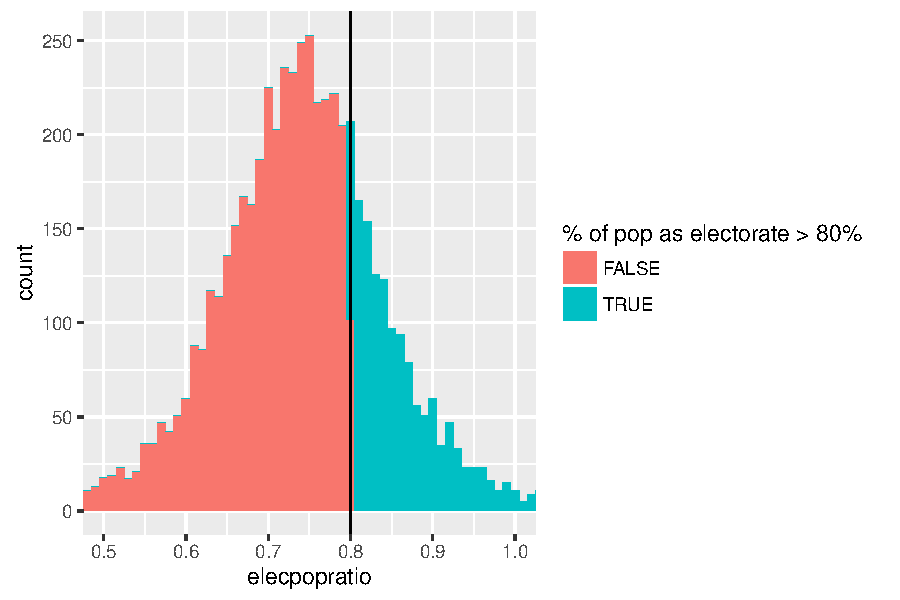
\includegraphics[width=\maxwidth]{figure/unnamed-chunk-11-1} 

\end{knitrout}

Seems like that the density is the same across the cutoff

\end{document}
